% ------------------------------------------------------------------------------------------------------------------------------------------------
\chapter{Cluster scaling and performance analysis}
\label{chap:perf-scalability}

This section will focus on analysing as well as presenting improvements to the cluster deployment which can and have been applied to the Hadoop cluster leveraged by the Analyser application presented in previous chapters.

In Section \ref{sec:scaling-hadoop} several challanges and typical problems with scaling Hadoop clusters will be presented, and then followed up by solutions applied during the work on this thesis.

Section \ref{sec:scaling-akka} will briefly explain scalability concerns related to an Akka based cluster deployment, yet as this component has not been as critical to overal system performance as the Analyser and Hadoop cluster, the Akka cluster has been deemed ''good enough'' for the scope of this paper.

\todo{explain what section does what}

% ------------------------------------------------------------------------------------------------------------------------------------------------
\section{Scaling Hadoop}
\label{sec:scaling-hadoop}
This section will focus on analysing and tuning the various settings of the Hadoop cluster deployed for the previously described Analyser application. Subsections focus on tuning the cluster on a setting--by--setting basis yet the tuning will always be enforced by a business need, which in this case will be represented as the need to speed up processing of the map reduce pipelines producing results which were explained in Chapter \ref{chap:analysis-examples}.

\subsection{Storing images on HDFS, while avoiding the ''Small Files Problem''}
\label{sec:sequence-files}
Most algorithms used in Oculus operate on a frame-by-frame basis, which means that it is most natural to store all data as ''data for frame 343 from movie XYZ''. This applies to everything from plain bitmap data of a frame to metrics such as histograms of colours of a given frame or other metadata like the extracted text content found in this frame.

Sadly this abstraction does \textit{not} work nicely with Hadoop, it would cause the well--known ''small-files problem'' which leads to \textit{major} performance degradation of the Hadoop cluster is left unadressed. This section will focus on explaining the problem and what steps have been taken to prevent it from manifesting in the presence of millions of ''frame-by-frame'' pieces of data.

Hadoop uses so called ''blocks'' as smallest atomic unit that can be used to move data between the cluster.
The default block size is set to \textit{64 megabytes} on most Hadoop distributions.

This also means that if the DFS takes a write of one file (assuming the \textit{replication factor} equals 1) it will use up one block. By itself this is not worrying, because other than in traditional (local) file systems such as EXT3 for example, when we store N bytes in a block on HDFS,
the the file system can still use block's unused space. Figure \ref{fig:no-sequence-file} shows the structure of a block storing only one frame of a movie.

\begin{figure}[ch!]
  \centering
  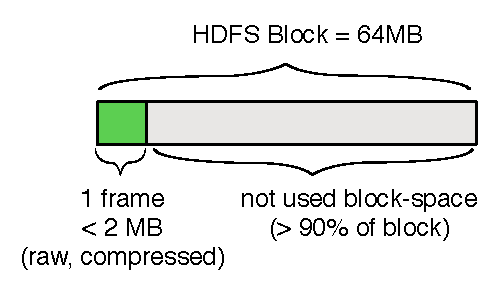
\includegraphics[scale=0.9]{diagrams/no-sequence-file.pdf}
  \caption{When storing a small file in HDFS, it still takes up an entire block. The grey space is not wasted on disk, but causes \textit{name-node} to store 1 block entry in memory.}
  \label{fig:no-sequence-file}
\end{figure}

The problem stemming from writing small files manifests not directly by impacting the used disk space, but in increasing memory usage in the clusters so called \textit{name-node}. The name-node is responsible for acting as a lookup table for locating the blocks in the cluster. Since name-node has to keep 150KB of metadata for each block in the cluster, creating more blocks than we actually need quickly forces the name-node to use so much memory, that it may run into long garbage collection pauses, degrading the entire cluster's performance. To put precise numbers to this -- if we would be able to store 500MB of data in an optimal way, storing them on HDFS would use 8 blocks -- causing the name node to use approximately 1KB of metadata. On the other hand, storing this data in chunks of 2MB (for example by storing each frame of a movie, uncompressed) would use up 250 HDFS blocks, which results in additional 36KB of memory used on the name-node, which is 4.5 times as much (28KB more) as with optimally storing the data! Since we are talking about hundreds of thousands of files, such waste causes a tremendous unneeded load on the name-node.

It should be also noted, that when running map-reduce jobs, Hadoop will by default start one map task for each block it's processing in the given Job. Spinning up a task is an expensive process, so this too is a cause for performance degradation, since having small files causes more \textit{Map tasks} being issued for the same amount of actual data Hadoop will spend more time waiting for tasks to finish starting and collecting data from them than it would have to.

% ------------------------------------------------------------------------------------------------------------------------------------------------
\subsubsection{Sequence Files}
\label{sequence-file}
The solution applied in the implemented system to resolve the small files problem is based on a technique called ''Sequence Files'', which are a manually controlled layer of abstraction on top of HDFS blocks. There are multiple Sequence file formats accepted by the common utilities that Hadoop provides \cite{hadoop-seq-files} but they all are \textit{binary header-prefixed key-value formats}, as visualised Figure \ref{fig:sequence-file}.


\begin{figure}[ch!]
  \centering
  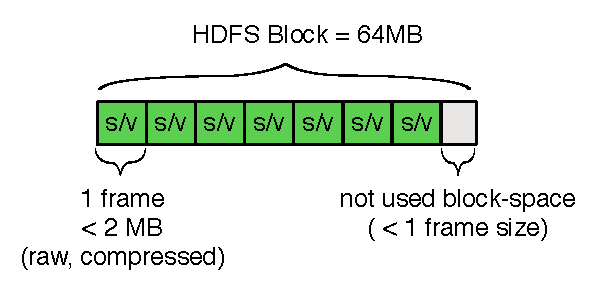
\includegraphics[scale=0.9]{diagrams/sequence-file.pdf}
  \caption{A SequenceFile allows storing of multiple small chunks of data in one HDFS Block.}
  \label{fig:sequence-file}
\end{figure}

Using Sequence Files resolves all previously described problems related to small files on top of HDFS. Files are no longer ''small'', at least in Hadoop's perception,
since access of frames of a movie is most often bound to access other frames of this movie we don't suffer any drawbacks from such storage format.

Another solution that could have been applied here is the use of HBase and it's key-value design instead of the explicit use of Sequence Files, yet this would not yield much performance nor storage benefits as HBase stores it's Table data in a very similar format as Sequence Files. The one benefit from using HBase in order to avoid the small files problem would have been random access to any frame, not to ''frames of this movie'', but since I don't have such access patterns and it would complicate the design of the system I decided to use Sequence Files instead.



% ------------------------------------------------------------------------------------------------------------------------------------------------
\subsection{Tuning replication factors}
\label{sec:tuning-replication-factors}
One of the many tuneable aspects of Hadoop deployments that can have a very high impact on the clusters performance is the \textit{replication factor}, which stands for ''the number of datanodes a piece of data is replicated to''. This section will explain in detail how a tuning this factor, and leveraging Hadoop's scheduling mechanisms can be tweaked to trade of storage space (higher replication factors) to faster execution times of jobs.

Hadoop's primary strength in big data applications lies within leveraging \textit{data locallity} whenever possible. The concept of data locallity means that instead of moving the data around in the cluster, to a node where the application is running, the Task Scheduler will try find such ''map slots'' (multiple such slots can be assigned to one data node) that the data the job needs to process will be local to the node the slot resides on. Effectively this means that application code (jar and class files) will be sent to the executing server, and not the inverse. The rationale behind this measure is that the amounts of data are way bigger than the size of applications in these kinds of systems -- thus, avoiding to move the data can save both costs and precious time.


\begin{figure}[ch!]
  \centering
  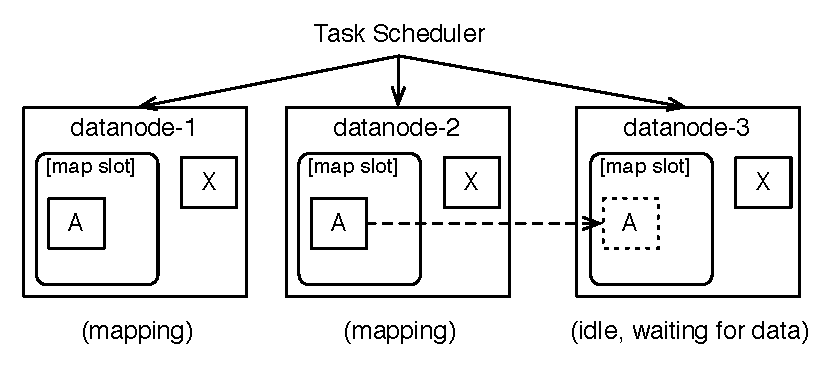
\includegraphics[width=\textwidth]{img/forced-data-replication.pdf}
  \label{fig:replication-ad-hoc}
  \caption{Three node cluster, with idle 3rd node; Scheduler will replicate data A while running the Job, in order to start a task requireing A on the 3rd idle node.}
\end{figure}


While data locallity is a \textit{priority} for the scheduler, it is by no means a hard requirement. In a scenario outlined in Figure \ref{fig:replication-ad-hoc} a job has been submitted to a 3-node cluster. The replication factor in the cluster is set to 2 -- which can be noticed by the number of times each piece of data is replicated among the datanodes. In the absence of any other jobs scheduled on the cluster, the fair--scheduler will decide to use the 3rd data node in order to accelerate the processing of the job, even though it does not have the required piece of data located on it (splits of A). Replicating the data over to datanode-3 is quite costly, and even though it may speed-up the total compute time, we loose time on transfering the data in an ad-hoc fashion.

By tweaking the replication factor for the given file, which we expect to be needed on more nodes, we can speed up the total compute time of a given job. In order to change the replication factor of a given path, one can use either the Java APIs or the hadoop command line tool, as shown in Listing \ref{lst:cli-change-replication}.

\begin{lstlisting}[caption={Explicitly changing the replication factor on a path using command line tools}, label={lst:cli-change-replication}]
hadoop dfs -setrep -R -w 3 /oculus/source/e98uKex3hSw.mp4.seq
\end{lstlisting}

By increasing the replication factor of paths that we know they will be used in many mappers, we can increase the number of data-local slots available to the scheduler, and avoid having to migrate the data in an ad-hoc fashion. Of course, the tradeoff is requireing even more disk space in the cluster, but it is well worth considering to raise the replication factor of a path while it is ''hot'', and lowering it afterwards.

\begin{figure}
  \centering
  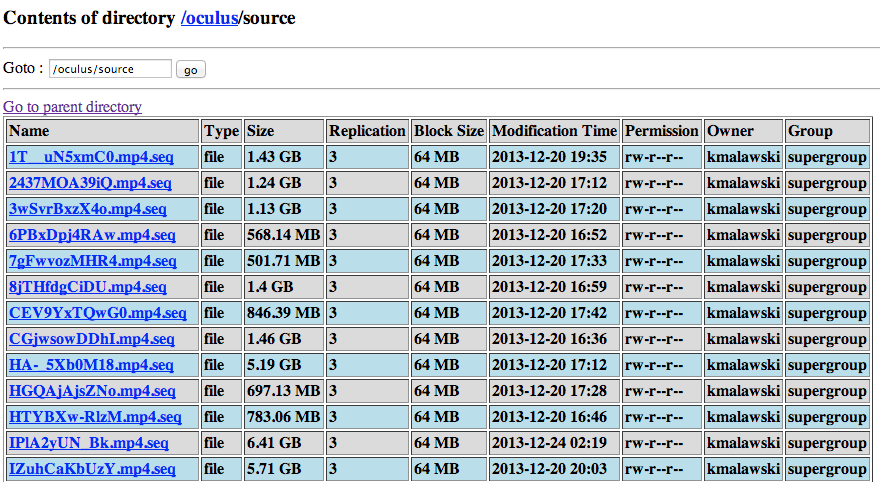
\includegraphics[width=\textwidth]{img/hadoop/hdfs_show-replication}
  \label{fig:hdfs-replication-factors}
  \caption{HDFS on-line browser, running on datanode (port: 50075)}
\end{figure}

The replication factor of a file (or path) is such an important value, it's usually always displayed along side any file listing within the Hadoop UIs (see Figure \ref{fig:hdfs-replication-factors}) as well as command line tools. It should also be noted that it is impossible to set the replication factor to a higher number than there are datanodes present in the cluster -- as the replication requirement would not be possible to be fulfilled (for obvious reasons).


\subsection{Tuning number of nodes}
\label{sec:tuning-number-of-nodes}



% ------------------------------------------------------------------------------------------------------------------------------------------------
\section{Scaling the Loader (actor system)}
\label{sec:scaling-akka}

\todo{scale it to more nodes...}
